\documentclass[12pt]{book}

\usepackage[margin=1.1in]{geometry}
\usepackage{amsmath, amssymb, mathtools}
\usepackage{tikz}
\usetikzlibrary{positioning}
\usepackage{enumitem}
\usepackage{xcolor}
\usepackage{mdframed}
\usepackage{epigraph}
\usepackage{booktabs}
\usepackage{array}
\usepackage[colorlinks=true, linkcolor=blue!50!black, citecolor=blue!50!black]{hyperref}

\setlength{\epigraphwidth}{0.85\textwidth}

\definecolor{mottoblue}{RGB}{235,242,250}
\definecolor{mottoline}{RGB}{70,110,160}

\newmdenv[
  backgroundcolor=mottoblue,
  linecolor=mottoline,
  linewidth=1pt,
  roundcorner=4pt,
  innertopmargin=10pt,
  innerbottommargin=10pt,
  innerleftmargin=12pt,
  innerrightmargin=12pt,
  skipabove=14pt,
  skipbelow=14pt
]{mottobox}

\newcounter{reflectq}
\newenvironment{reflectquestions}
  {\begin{list}{\textbf{\arabic{reflectq}.}}
    {\usecounter{reflectq}\setlength{\leftmargin}{1.6em}\setlength{\itemsep}{6pt}}}
  {\end{list}}

\begin{document}

\setcounter{chapter}{1}

\chapter[Understanding Versus Measurement]{Understanding Versus Measurement: Why Physics Is Not Data Science}
\label{ch:understanding}

\begin{mottobox}
\noindent\textit{Not being able to define a thing precisely is not the same failure as not understanding it.}

\vspace{4pt}
\noindent\small Chapter~1 showed that physics survives without precise definitions because it replaces them with measurement procedures. This chapter argues that measurement procedures are the \emph{floor} of physics, not its ceiling --- and that the gap between the floor and the ceiling is exactly what separates a physicist from a curve-fitting algorithm.
\end{mottobox}

\section{Two Sentences That Get Merged}
\label{sec:two-sentences}

The claim in the epigraph above rests on two sentences Feynman actually said, in different lectures, about different things -- and they are routinely collapsed into one. They should not be.

``We cannot define anything precisely'' was said about ordinary words like \emph{motion} -- a confession that physics does not wait for philosophical certainty about what a thing \emph{is} before it starts measuring it precisely\footnote{See Chapter~1, \S1.2, and R.~P.~Feynman, R.~B.~Leighton, and M.~Sands, \emph{The Feynman Lectures on Physics}, Vol.~I, Ch.~8, \S8.1.}. That is an epistemic strategy: start with measurement, because measurement is checkable and definition-by-essence is not.

``I think I can safely say that nobody understands quantum mechanics'' was said in a completely different spirit, in the sixth of Feynman's 1964 Messenger Lectures at Cornell\footnote{R.~P.~Feynman, \emph{The Character of Physical Law} (BBC/MIT Press, 1965), Lecture 6, ``Probability and Uncertainty: The Quantum Mechanical View of Nature.''}. Feynman had just finished pointing out that although newspapers once claimed only twelve people understood relativity, that was never really true --- once Einstein's paper was published, plenty of people came to understand it, in the ordinary sense of being able to picture what it says. Quantum mechanics, he then says, is different: nobody has ever been able to reduce it to a picture built out of everyday experience, the way you can eventually picture curved spacetime with enough effort. That is not a statement that physicists cannot use quantum mechanics, predict with it, or reason about it --- they do all three, correctly, every day, and Feynman himself spent the rest of that same lecture doing exactly that. It is a much narrower claim: no one has found a \emph{classical, intuitive mechanism} underneath it. Understanding, in that specific and demanding sense, is missing. Understanding in the working sense --- knowing the structure, deriving its consequences, trusting it enough to build a transistor or a laser on top of it --- is not.

This chapter is about the difference between those two kinds of understanding, and about a claim worth taking seriously: that pure operationalism, on its own, cannot tell them apart. If all that mattered were successful measurement and prediction, there would be no principled way to say that a physicist understands gravity more deeply than a weather-prediction algorithm understands rain. Physics needs, and has, a further standard.

\section{What Operationalism Leaves Out}
\label{sec:blind-spot}

Return to Chapter~1's account of measurement. An operational definition says: a quantity is whatever a specified procedure outputs. This is enough to make a concept scientific --- checkable, shareable, free of unfalsifiable metaphysics. It is not enough, on its own, to distinguish two very different kinds of success.

\begin{enumerate}
\item A theory that predicts a measurement because it encodes something structural about how the world is put together: a small number of principles from which the measured value can be \emph{derived}.
\item A model that predicts a measurement because it has been fitted, with enough free parameters, to enough past instances of that same measurement, with no claim about structure at all.
\end{enumerate}

Both can satisfy the operationalist's only stated requirement: the output matches what the ruler, clock, or detector reads. Bridgman's operationalism, taken as a complete philosophy of physics rather than as a starting discipline, has no vocabulary for preferring one over the other. Yet every working physicist does prefer one over the other, strongly and immediately. The rest of this chapter tries to say, precisely, why.

\section{Three Ways to Say the Same Thing}
\label{sec:three-ways}

The clearest demonstration Feynman ever gave of this distinction was not a slogan; it was a worked example, in the second of the same 1964 lectures\footnote{Feynman, \emph{The Character of Physical Law}, Lecture 2, ``The Relation of Mathematics to Physics.''}. He points out that Newton's law of gravitation can be written in at least three completely different-looking forms.

\begin{description}[leftmargin=1.4em, style=nextline]
\item[Action at a distance.] Each mass reaches out across empty space and pulls on every other mass directly:
\[
  F = \frac{G m_1 m_2}{r^2}.
\]
\item[The field method.] Every mass creates a field filling all of space; a second mass simply responds to the local field value at its own location, with no need to reach anywhere:
\[
  \nabla^2 \phi = 4\pi G \rho, \qquad \vec F = -m\,\nabla \phi.
\]
\item[The principle of least action.] Of all the conceivable paths a particle could take between two points, nature selects the one that makes a particular quantity, the action $S$, stationary:
\[
  \delta S = \delta\!\int (T - V)\, dt = 0.
\]
\end{description}

For every experiment classical mechanics can perform, these three formulations issue identical predictions. Bridgman's yardstick sees no difference between them at all: same measurement in, same number out, for all three, always. And yet, as Feynman insists, they are not the same idea wearing different clothes. They organize your intuition differently, suggest different questions, and --- this is the decisive part --- they are not equally good starting points for the \emph{next} theory.

When physics moved from classical to quantum mechanics, the action-at-a-distance picture and the field-at-a-point picture both had to be abandoned or radically reworked. The least-action formulation, by contrast, generalized almost gracefully: Feynman's own path-integral formulation of quantum mechanics, developed in 1948, is built by summing a phase $e^{iS/\hbar}$ over every conceivable path, weighting the classical path of least action as the one that survives in the limit $\hbar \to 0$\footnote{See \emph{The Feynman Lectures on Physics}, Vol.~II, Ch.~19, ``The Principle of Least Action.''}. Three formulations, operationally indistinguishable in 1687 and still operationally indistinguishable today for any classical experiment --- but only one of them was carrying the structure that quantum mechanics needed. Operational equivalence in the old domain said nothing at all about generative power in the new one.

That gap is what \emph{understanding} means in physics. It is not merely getting today's number right. It is possessing a formulation with enough internal structure that it tells you, in a principled way, what to try next.

\begin{figure}[ht]
\centering
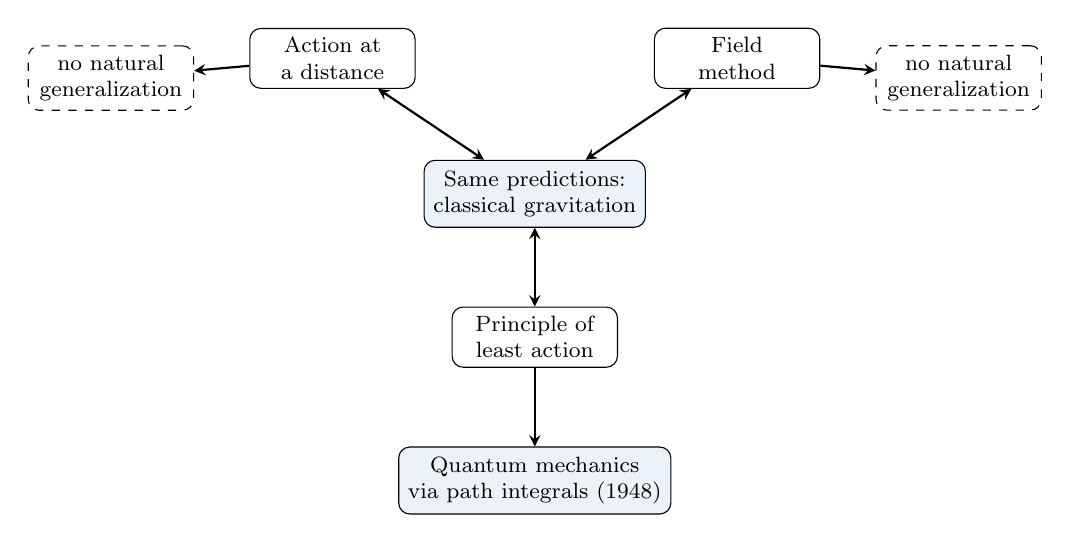
\begin{tikzpicture}[every node/.style={font=\footnotesize}, >=stealth]
  \node[draw, rounded corners, fill=mottoblue, minimum width=2.7cm, minimum height=0.85cm, align=center] (center)
    {Same predictions:\\ classical gravitation};

  \node[draw, rounded corners, minimum width=2.1cm, minimum height=0.75cm, align=center, above left=0.9cm and 0.1cm of center] (force) {Action at\\ a distance};
  \node[draw, rounded corners, minimum width=2.1cm, minimum height=0.75cm, align=center, above right=0.9cm and 0.1cm of center] (field) {Field\\ method};
  \node[draw, rounded corners, minimum width=2.1cm, minimum height=0.75cm, align=center, below=1.0cm of center] (action) {Principle of\\ least action};

  \draw[<->, thick] (force) -- (center);
  \draw[<->, thick] (field) -- (center);
  \draw[<->, thick] (action) -- (center);

  \node[draw, dashed, rounded corners, minimum width=2.1cm, minimum height=0.65cm, align=center, left=0.7cm of force, yshift=-0.25cm] (deadforce) {no natural\\ generalization};
  \node[draw, dashed, rounded corners, minimum width=2.1cm, minimum height=0.65cm, align=center, right=0.7cm of field, yshift=-0.25cm] (deadfield) {no natural\\ generalization};
  \node[draw, rounded corners, fill=mottoblue, minimum width=2.9cm, minimum height=0.85cm, align=center, below=1.0cm of action] (qm) {Quantum mechanics\\ via path integrals (1948)};

  \draw[->, thick] (force) -- (deadforce);
  \draw[->, thick] (field) -- (deadfield);
  \draw[->, thick] (action) -- (qm);
\end{tikzpicture}
\caption{Three formulations of Newton's law of gravitation, operationally identical for every classical measurement --- yet only the least-action formulation carried the structure needed to generalize to quantum mechanics. Operational equivalence in one domain does not imply equal understanding, or equal reach.}
\label{fig:three-ways}
\end{figure}

\section{What Understanding Buys You}
\label{sec:what-it-buys}

The philosopher and computer scientist Judea Pearl has proposed a useful vocabulary for the same distinction, developed for a very different purpose: distinguishing statistical, correlational reasoning from causal reasoning\footnote{J.~Pearl and D.~Mackenzie, \emph{The Book of Why: The New Science of Cause and Effect} (Basic Books, 2018).}. He describes three rungs of a ladder.

\begin{center}
\begin{tabular}{@{}>{\raggedright\arraybackslash}p{2.6cm} >{\raggedright\arraybackslash}p{4.6cm} >{\raggedright\arraybackslash}p{4.6cm}@{}}
\toprule
\textbf{Rung} & \textbf{Typical question} & \textbf{What answers it} \\
\midrule
Association & What does a value of $X$ tell me about $Y$? & A fit to past data; correlation \\
Intervention & What happens to $Y$ if I \emph{change} $X$? & A causal / mechanistic model \\
Counterfactual & What would $Y$ have been, had $X$ been different? & A model that supports reasoning beyond any data actually collected \\
\bottomrule
\end{tabular}
\end{center}

A purely operational, purely data-fitted model can climb no higher than the first rung by construction: it was built to reproduce association between measurement and measurement, and nothing in its construction licenses a claim about what would happen under conditions it has never seen. A physical theory with real structure --- Newton's law derived from a principle, not merely fitted to Tycho Brahe's tables --- operates on the second and third rungs almost as a matter of course. It tells you what happens if you double the mass of the Sun, a question no data set has ever answered, because the answer is derivable rather than looked up.

History supplies the record of this pay-off. The existence and orbit of Neptune were predicted, in 1846, from irregularities in Uranus's orbit, before anyone pointed a telescope at the right patch of sky. The positron was predicted by Dirac's equation in 1928, purely from requiring the equation to be consistent, four years before one was observed in a cloud chamber. Gravitational waves were predicted in 1916 and detected almost exactly a century later, in 2015, with the detected waveform matching the theoretical prediction for two merging black holes to remarkable precision. None of these were interpolations inside a training set. Each was an extrapolation, licensed by structure, into territory no measurement had ever visited --- exactly the kind of claim Pearl's first rung cannot support, and exactly what physicists mean when they say they \emph{understand} gravity, or the electron, rather than merely being able to predict its next measured value.

\section{Physics and Data Science}
\label{sec:data-science}

This is the precise place where physics and data science part ways, and it is worth stating the comparison without exaggerating it in either direction.

Train a sufficiently flexible statistical model on centuries of recorded planetary positions and it will predict tomorrow's positions beautifully --- quite possibly to a precision rivaling Newton's own equations, for exactly the regime it was trained on. It has, in the fullest operational sense, learned to measure and predict planetary motion. What it has not done is acquire a reason to trust its own output the moment the situation changes: a new comet on a hyperbolic orbit, a spacecraft under active thrust, a binary star system where the gravitational field is far stronger than anything in the training data. A model built on correlation has no internal signal that it has left its depth --- it will output a confident number regardless. Newton's law, by contrast, comes with a built-in, structural account of exactly where and why it should be expected to fail: at speeds approaching $c$, or fields strong enough that spacetime curvature can no longer be neglected. Knowing your own boundary of validity is itself a form of understanding, and it is precisely what falls out of having a mechanism rather than a fit.

None of this makes data-driven methods unscientific, and it would be a mistake to read this chapter that way. Statistical inference is indispensable precisely where no mechanistic theory yet exists, and some of the most interesting current work in physics itself uses machine learning as a tool for discovery --- to search for patterns in particle-collider data, or in gravitational-wave signals, that a human physicist might not think to look for. Tellingly, though, the most physically successful of these tools are increasingly built to encode known structure directly --- conservation laws, symmetries, the least-action principle itself --- rather than learning everything from scratch. That design choice is itself an admission of this chapter's argument: bare correlation extrapolates badly, and the fix physicists reach for is always the same one Feynman reached for in 1948 --- find the formulation that carries structure, not just the one that fits the numbers.

\section{Restoring the Motto}
\label{sec:restoring}

Chapter~1 ended with a motto built from three of Feynman's remarks: physics does not need to know what space, time, or motion \emph{are}, only how to measure them. That motto is correct as far as it goes, and it is where physics has to start. This chapter has argued that it is not where physics is content to stop.

A physicist who has only an operational definition and an accurate prediction has done real, indispensable work --- exactly the work Chapter~1 celebrated. A physicist who additionally has a structure --- a small set of principles from which that prediction, and a thousand others never yet measured, can all be derived --- has done something further, and it is that further thing which earns the word \emph{understand}. The motto of this chapter is the necessary second half of the first:

\begin{mdframed}[backgroundcolor=gray!8, linecolor=gray!40, linewidth=0.6pt, roundcorner=3pt]
\centering
\textit{We measure a thing before we understand it. We understand it once our account of it lets us predict what we have never measured at all.}
\end{mdframed}

\bigskip
\noindent\textbf{Reflection Questions}
\begin{reflectquestions}
\item Feynman's three formulations of gravitation give identical predictions for every classical experiment. Propose your own criterion --- besides ``it generalized to quantum mechanics,'' which we only know with hindsight --- that a physicist in 1687 could plausibly have used to prefer one formulation over another.
\item Explain, in your own words, why Feynman's remark that nobody understands quantum mechanics is compatible with quantum mechanics being an extremely well understood theory in the working, predictive sense.
\item Give an example, from any field, of a prediction that was later confirmed and that could only have come from a structural model, not from fitting a curve to past data. What would have had to go wrong for a pure correlation to produce the same successful prediction by accident?
\item A weather-forecasting model and a climate model can both be built from partly the same physics (fluid dynamics, thermodynamics) and partly statistical fitting. Which parts of each model do you expect to extrapolate reliably decades into a changing climate, and which parts do you expect to break down? Why?
\item Is it possible, even in principle, for a purely data-driven model to climb to Pearl's second or third rung without any hand-built physical structure? What would you need to give it?
\end{reflectquestions}

\bigskip
\begin{thebibliography}{9}

\bibitem{feynmancpl}
R.~P.~Feynman, \emph{The Character of Physical Law} (BBC/MIT Press, 1965), Lectures 2 and 6.

\bibitem{feynmanlectures2}
R.~P.~Feynman, R.~B.~Leighton, and M.~Sands, \emph{The Feynman Lectures on Physics}, Vol.~II, Ch.~19, ``The Principle of Least Action,'' and Vol.~I, Ch.~8.
\url{https://www.feynmanlectures.caltech.edu/}

\bibitem{pearl}
J.~Pearl and D.~Mackenzie, \emph{The Book of Why: The New Science of Cause and Effect} (Basic Books, 2018).

\bibitem{bridgman2}
P.~W.~Bridgman, \emph{The Logic of Modern Physics} (Macmillan, 1927).

\end{thebibliography}

\end{document}
